% Compile with XeLaTeX or LuaLaTeX
\documentclass[12pt,a4paper]{article}
\usepackage{xcolor}
\usepackage{titlesec}
\usepackage{fontspec}
\defaultfontfeatures{Mapping=tex-text}
\usepackage{xunicode}
\usepackage{xltxtra}
\usepackage{polyglossia}
\usepackage{indentfirst}             % 段首缩进

\setdefaultlanguage{english}

% 设置字体
\setsansfont{Calibri}
\setmainfont[BoldFont=SimHei]{STKaiti}
\usepackage{amsmath}
\usepackage{amsfonts}
\usepackage{amssymb}
\usepackage{graphicx}
\usepackage{float}
\usepackage{abstract}
% 设置页边距
\usepackage[left=2cm,right=2cm,top=2cm,bottom=2cm]{geometry}

% 新定义字体
\newfontfamily\song{STKaiti}          % 宋体
\newfontfamily\hei{STKaiti}           % 黑体
\XeTeXlinebreaklocale "zh"           % 中文断行

% Define light and dark Microsoft blue colours
\definecolor{MSBlue}{rgb}{.0,.0,.0}
\definecolor{MSLightBlue}{rgb}{.0,.0,.0}
% Define a new fontfamily for the subsubsection font
% Don't use \fontspec directly to change the font
\newfontfamily\subsubsectionfont[Color=MSLightBlue]{Times New Roman}
% Set formats for each heading level
\titleformat*{\section}{\Large\bfseries\sffamily\color{MSBlue}\song}
\titleformat*{\subsection}{\large\bfseries\sffamily\color{MSLightBlue}\song}
\titleformat*{\subsubsection}{\itshape\subsubsectionfont\song}

\author{黄红清\footnote{email: huanghqdx@163.com\quad phone:18069875273\quad date:2018.5.4}\quad21721214\\[2ex] 浙江大学计算机学院\\[2ex]}
\title{生物智能算法课程报告--鲸鱼优化算法}
\date{}
\begin{document}

%%%% 段落首行缩进两个字 %%%%
\makeatletter
\let\@afterindentfalse\@afterindenttrue
\@afterindenttrue
\makeatother
\setlength{\parindent}{2em}  %中文缩进两个汉字位
\maketitle

\begin{abstract}
\renewcommand{\abstractname}{摘要}
本文对Seyedali Mirjalili等人提出的鲸鱼优化算法进行了比较深入浅出的阐述,从算法的灵感来源、模型建立到伪代码实现都进行了更加详细地分析和叙述。本文还设计了该算法的可视化模拟程序,通过在二维空间搜索4个典型的凸函数和非凸函数的最优解,来直观地分析和理解鲸鱼优化算法的位置变换策略和搜索过程,给出了对鲸鱼优化算法的主观评价。
\end{abstract}

\section{引言}
鲸鱼优化算法(Whale Optimization Algorithm , WOA)是由Seyedali Mirjalili等人在2016年提出的一种基于群聚的生物智能算法,通过模拟座头鲸鱼群捕食磷虾的行为,建模出了鲸鱼优化算法来解决各类优化问题。

从生物的角度看,从鲸鱼的捕食行为获取生物智能优化算法是非常合情合理的。因为鲸鱼是一种非常神奇的生物,他们被认为是高度聪明的动物,且有着像人类一样的感情,已被证明鲸鱼在大脑的某些区域有和人类的梭形细胞相似的细胞,而这些细胞恰恰负责人类的决策、情绪和社会行为。鲸鱼的聪明正是因为他们有人类两倍的这种梭形细胞,他们可以像人类一样思考、学习、决策、社交(拥有一生的家庭),甚至拥有情感并产生自己的方言,只不过这些行为的程度比人类低级许多。

鲸鱼优化算法是根据座头鲸捕食磷虾的行为来建模的,座头鲸捕食磷虾主要是通过向上螺旋制造起泡网的方式来进行的。
\begin{figure}[H]
\centering
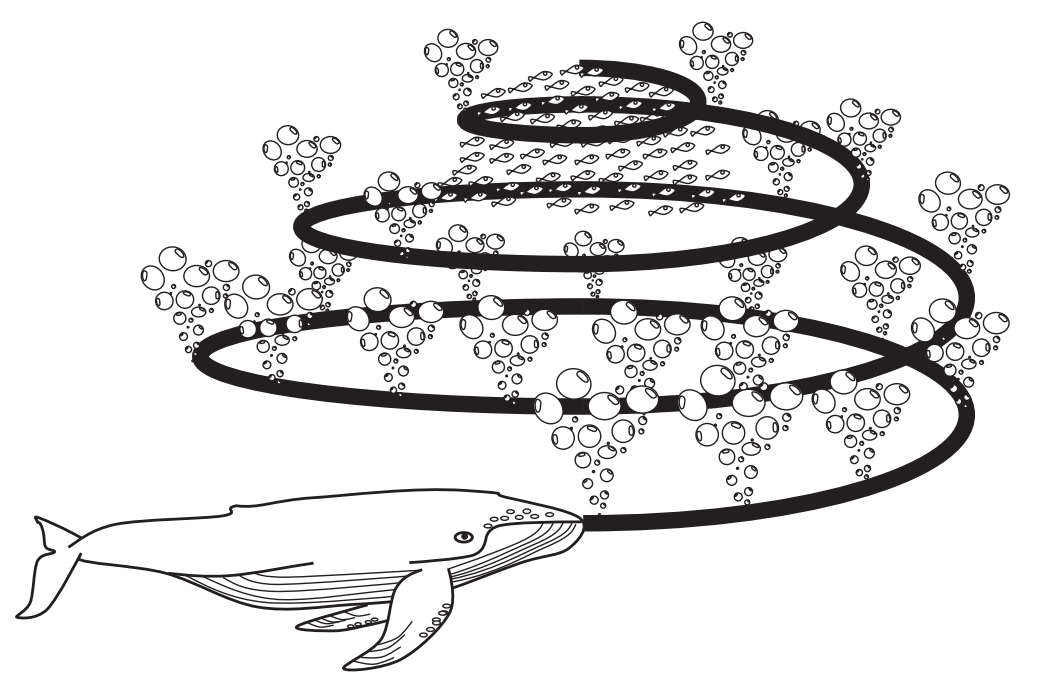
\includegraphics[width=0.5\textwidth]{figure/bubble_net.png}
\renewcommand\figurename{图}\caption{座头鲸用气泡网捕食磷虾群}
\end{figure}
如图1所示,一只座头鲸在捕食磷虾时,首先下潜到水下12米的位置,开始不断制造起泡,并按照螺旋形状朝着水面游动。这些气泡像一张不断收缩的大网,使磷虾群就不断被起泡逼迫到一个很小的区域,此时座头鲸垂直向磷虾群游去,捕食它们。

鲸鱼优化算法就是利用多条鲸鱼,将磷虾群当做局部最优解,鲸鱼所在位置当做当前搜索的解的位置,朝着局部最优解按螺旋或包围收缩变换位置,发现更好的解来更新局部最优解,反复向新的局部最优解搜索,尽可能地搜索到全局最优解。

\section{算法模型}
注:本文公式在编号时,采用了与原论文一致的编号以方便拿原论文进行参照理解。

直观上讲,鲸鱼优化算法就是在一个优化问题的解空间中,不断朝着局部最优解的方向,以某种方式迭代变换当前搜索位置,不断找出更优解的过程。作者将算法分为了两个阶段,分别是开发阶段和探索阶段。

在开发阶段,分别按照包围收缩和螺旋形朝着局部最优解的方向更新位置,在更新的过程中,每遇到比局部最优解更好的解,就把它作为当前的局部最优解,朝着它不断更新位置。这一阶段的主要目的是尽可能穷尽搜索当前局部最优解附近的更好的解,即尽可能更完全地开发当前局部最优解附近的更好的解。

在探索阶段,按照包围收缩的方式朝着随机选定的一个位置收缩更新位置,同样在更新的过程中,用新的局部最优解代替旧的局部最优解,但探索阶段始终朝着随机位置更新搜索位置。这一阶段的主要目的是避免搜索过程陷入局部最优,补足了开发阶段的短板。

\subsection{开发阶段--包围收缩位置建模}
鲸鱼优化算法假定全局最优解靠近局部最优解,于是便可以向着局部最优解不断收缩位置,查找更好的解。包围收缩阶段的模型用公式表示如下:
\begin{displaymath} \vec{D}= \left | \vec{C}\cdot\vec{X^{*}}(t)-\vec{X}(t) \right | \eqno(2.1)  \end{displaymath}
\begin{displaymath} \vec{X}(t+1)=\vec{X^{*}}(t)-\vec{A}\cdot \vec{D} \eqno(2.2)  \end{displaymath}

其中,$t$代表当前的迭代次数;$\vec{A}$和$\vec{C}$是系数向量;$\vec{X^*}$是当前搜索到的局部最优解的位置(坐标);$\vec{X}$是当前鲸鱼所处的搜索位置;||是绝对值运算(即将向量中的负数都变成非负数);$\cdot$是向量的对应元素相乘;这里的$\vec{X^*}$在搜索过程中是不断更新的最优解。

向量$\vec{A}$和向量$\vec{C}$的计算方式如下:
\begin{displaymath} \vec{A}=2\vec{a}\cdot\vec{r}-\vec{a} \eqno(2.3)\end{displaymath}
\begin{displaymath} \vec{C}=2\cdot\vec{r} \eqno(2.4)\end{displaymath}

其中,$\vec{a}$是一个从2到0线性递减的向量;$\vec{r}$是0到1之间的随机向量。

我们结合二维搜索空间下的位置变化情况来理解包围收缩变换的公式。
\begin{figure}[H]
\centering
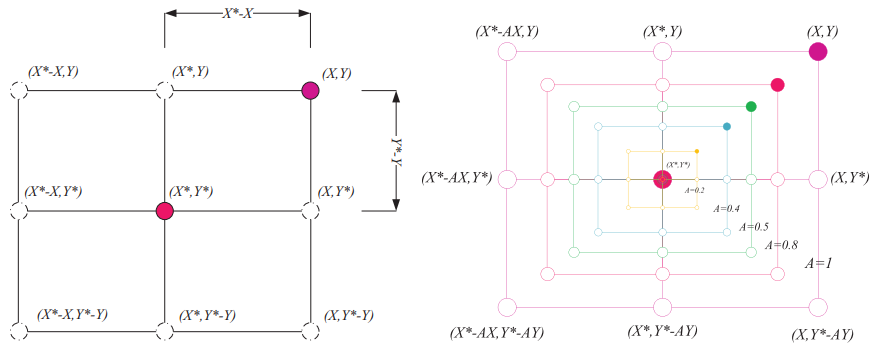
\includegraphics[width=1.0\textwidth]{figure/encircling.png}
\renewcommand\figurename{图}\caption{包围收缩的二维位置变换示意图}
\end{figure}

我们先看图2左图,首先对2.1式忽略系数向量$\vec{C}$,那么$\vec{D}$其实就是当前所在位置$(X,Y)$和局部最优位置$(X^*,Y^*)$之间的坐标差的绝对值向量,再对2.2式忽略系数$\vec{A}$,那么下次迭代搜索的位置就是当前局部最优位置减去坐标差的绝对值,即相对于$(X^*,Y^*)$左下角的固定位置。

为了使下次搜索位置能在相对于$(X^*,Y^*)$的一个包围圈上变换,就用到了系数$\vec{A}$,$\vec{A}$中的$\vec{r}$是0到1之间,因此$\vec{A}$就在$[-\vec{a},\vec{a}]$之间,可见$\vec{A}$向量每个元素的符号都是随机生成的,那么它与坐标差的绝对值向量进行对应元素相乘后,实际的坐标差向量中每个元素符号都会随机生成,下次迭代的位置就不会固定在左下角了,而是各个方向都有可能。

最后再看图2右图,当$\vec{a}$如果从1变为0时(从2到1在探索阶段再考虑),不管随机向量$\vec{r}$如何变,$\vec{A}\cdot \vec{D}$都呈现总体变小的趋势,即实现了收缩到局部最优解的目标。再回过头来看$\vec{C}$向量,实质上就是对当前最优位置进行了随机的波动,以增加位置更新的随机性,以更好地开发局部最优解附近的位置。

\subsection{开发阶段--螺旋更新位置建模}
螺旋更新搜索位置的公式如下:
\begin{displaymath} \vec{X}(t+1)=\vec{{D}'}\cdot e^{bl}\cdot cos(2\pi l)+\vec{X^{*}}(t) \eqno(2.5)\end{displaymath}

此处的$\vec{{D}'}=|\vec{X^{*}}(t)-\vec{X}(t)|$是局部最优位置和当前鲸鱼所在搜索位置的坐标差的绝对值;$e^{bl}$是对数螺线的定义,指螺线相对圆心位置成指数倍增长;$b$是定义螺旋形状的常数;$l$是-1到1之间的随机数。

螺旋搜索的过程如图3所示,同样是用二维平面的一个例子解释。
\begin{figure}[H]
\centering
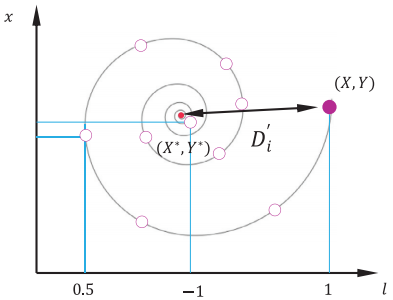
\includegraphics[width=0.4\textwidth]{figure/spiral.png}
\renewcommand\figurename{图}\caption{螺旋线更新位置的二维位置变换示意图}
\end{figure}

从公式${D}'\cdot e^{bl}$可以看出,下次迭代位置与当前最优位置坐标上的差距是指数趋势变化的。如果没有后面的$cos(2\pi l)$项,那么下一次迭代搜索的位置总在$X^*$最优位置的右上方,因为所有值都是非负的。于是增加$cos(2\pi l)$系数来让坐标差的绝对值向量每个元素符号随机变化,以搜索到最优位置附近螺旋线上每个方向的解空间。

至此,已经对两种开发阶段变换位置的方式进行了解释,需要注意的是,包围收缩变换位置是从外向内收缩变换的,而螺线变换位置由于没有$\vec{A}$系数,因此向里还是向外随机选定的。这两种方式作者分别按照0.5的概率来采取,用于更新下一代的迭代位置。用公式表示如下:
\begin{displaymath}
\vec{X}(t+1)=\begin{cases}
\vec{X^{*}}(t)-\vec{A}\cdot \vec{D} & \text{ if } p<0.5 \\ 
\vec{{D}'}\cdot e^{bl}\cdot cos(2\pi l)+\vec{X^{*}}(t) & \text{ if } p\geq 0.5 
\end{cases}
\eqno(2.6)\end{displaymath}

其中$p$是概率,$p$小于0.5时,采取包围收缩的方式更新位置,当$p$不小于0.5时,采取螺旋线更新位置的方式更新搜索位置。

\subsection{探索阶段--随机包围收缩位置建模}
2.1和2.2中介绍的位置更新策略都是根据当前搜索到的局部最优解的位置进行迭代位置更新的,这种搜索方式所能找到的最优解非常依赖于初始搜索到的局部最优位置,且搜索过程中不容易跳出当前局部最优解的附近范围。因此,需要引入跳出局部最优解的方法,就是随机包围收缩位置,这种策略同样克服了搜索结果过分依赖初始位置的缺点。

随机包围收缩位置的公式如下:
\begin{displaymath} \vec{D}=|\vec{C}\cdot \vec{X}_{rand}-\vec{X}| \eqno(2.7)\end{displaymath}
\begin{displaymath} \vec{X}(t+1)=\vec{X}_{rand}-\vec{A}\cdot \vec{D} \eqno(2.8)  \end{displaymath}

公式与包围收缩位置的公式几乎相同,只不过把原来的X*换成了随机选定的一个位置$\vec{X}_{rand}$,此时就用到了$\vec{A}$从2到1的变化情况,作者设计在$\vec{A}$从2到1变化时,随机选定$\vec{X}_{rand}$位置,向这个随机位置包围收缩更新位置,不断搜索新的最优解。而$\vec{A}$从1变到0时,只是朝着局部最优解包围收缩,因此并没有包围收缩得很非常靠近随机位置。
\begin{figure}[H]
\centering
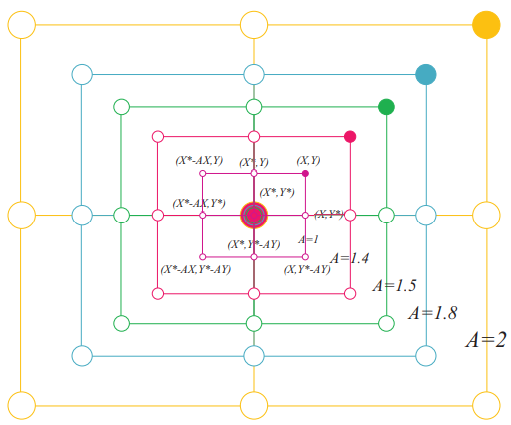
\includegraphics[width=0.4\textwidth]{figure/exploration.png}
\renewcommand\figurename{图}\caption{探索阶段随机包围的二维位置变换示意图}
\end{figure}

图4是$\vec{A}$在2到1过程中,按随机包围收缩更新位置的方式,朝着随机位置$\vec{X}_{rand}$(图中的$(X^*,Y^*)$)包围收缩搜索更优解的过程,当$\vec{A}$从1到0时,就不这么继续搜索了,而是继续回到2.1公式的收缩包围机制来更新位置。

\section{算法步骤}
鲸鱼优化算法的伪代码步骤如下:

Initialize\ the\ whales\ population\ $X_{i}$ (i = 1, 2, ..., n)

 Calculate\ the\ fitness\ of\ each\ search\ agent
 
 $X^{*}$=the\ best\ search\ agent
 
 \textbf{\emph{while}} (t < maximum\ number\ of\ iterations)
 
 \qquad \textbf{\emph{for}}\ each\ search\ agent
 
 \qquad Update\ a, A, C, l, and\ p
 
 \qquad \qquad \textbf{\emph{if1}} (p<0.5)
 
 \qquad \qquad \qquad \textbf{\emph{if2}} (|A| < 1)
 
 \qquad \qquad \qquad \qquad Update\ the\ position\ of\ the\ current\ search\ agent\ by\ the\ Eq. (2.2)
 
 \qquad \qquad \qquad \textbf{\emph{else if2}} ($|A|\geq 1$)
 
 \qquad \qquad \qquad \qquad Select\ a\ random\ search\ agent ($X_{rand}$)
 
 \qquad \qquad \qquad \qquad Update\ the\ position\ of\ the\ current\ search\ agent\ by\ the\ Eq. (2.8)
 
 \qquad \qquad \qquad \textbf{\emph{end if2}}
 
 \qquad \qquad \textbf{\emph{else if1}} ($p\geq  0.5$)
 
 \qquad \qquad \qquad Update\ the\ position\ of\ the\ current\ search\ by\ the\ Eq. (2.5)
 
 \qquad \qquad \textbf{\emph{end if1}}
 
 \qquad \textbf{\emph{end for}}

 \qquad Check\ if\ any\ search\ agent\ goes\ beyond\ the\ search\ space\ and\ amend\ it
 
 \qquad Calculate\ the\ fitness\ of\ each\ search\ agent
 
 \qquad Update\ $X^{*}$\ if\ there\ is\ a\ better\ solution
 
 \qquad $t=t+1$
 
 \textbf{\emph{end while}}
 
 return X*
 
 初始时,随机初始化一群鲸鱼(初代的搜索位置),计算每个位置的适应度选择出局部最优位置X*。在之后循环的过程中,每次都要更新这个X*成为当前搜索到的局部最优的位置。
 
在循环迭代过程中,对每个鲸鱼(搜索位置)按2中介绍的公式计算$\vec{a}$,$\vec{A}$,$\vec{C}$,$l$和$p$。当$p$小于0.5时,根据$\vec{A}$大于1还是小于1分别选择2.1式的包围收缩方式和2.8式的随机包围收缩方式更新这个鲸鱼的位置;当$p$大于0.5时,按2.5的螺旋更新位置方式更新该鲸鱼的位置。每次更新完位置后,首先对不合法的位置进行修正,然后计算每个鲸鱼新位置的适应度,更新最优解的位置到$X^*$,并使迭代代数$t+1$。

当迭代代数t达到最大代数时,结束搜索过程,返回当前最优的$X^*$作为最终的解。

\section{实验模拟}
本文利用OpenCV设计了一个可视化的在二维空间上搜索最优解的模拟程序,来直观地模拟展示鲸鱼优化算法的搜索过程,实际上,利用该程序可以模拟任何三维曲面在二维空间利用WOA算法搜索最优值的过程,本文分别以一个凸函数和一个凹函数来直观展示WOA的搜索过程,来对鲸鱼优化算法有个直观的理解。

每幅图中,白色方框代表当前的局部最优值,周围的白色圆点代表所有鲸鱼所在的当前位置。

\subsection{包围收缩和螺旋更新位置模拟结果}
在本节中,通过WOA求解$f(x)=x_1^2+x_2^2$在$x_1$、$x_2$属于[-1,1]间的最小值,把当前最优解固定在(0,0)处,$\vec{a}$值从1开始递减,来分别展示收缩包围和螺旋更新位置的两种策略。通过修改算法中的$p$和$\vec{a}$,设置当前局部最优解为最优解(0,0),来将循环中的判断条件控制在包围收缩操作上,来模拟50条鲸鱼包围收缩向中心的过程,每次迭代的鲸鱼位置模拟结果如下。
\begin{figure}[H]
\centering
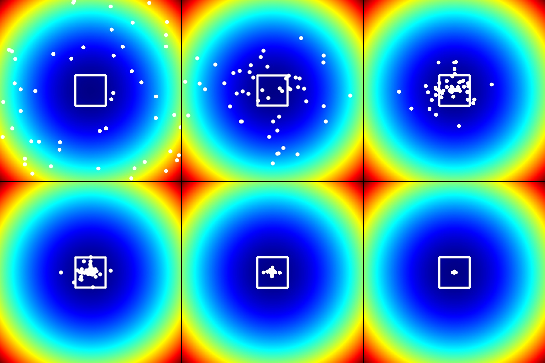
\includegraphics[width=0.75\textwidth]{figure/a.png}
\renewcommand\figurename{图}\caption{朝着中心包围收缩位置变换模拟结果}
\end{figure}

图5是包围收缩的迭代过程,由此可见,包围收缩更新位置策略能让周围的鲸鱼迅速向中央的局部最优值靠拢。
\begin{figure}[H]
\centering
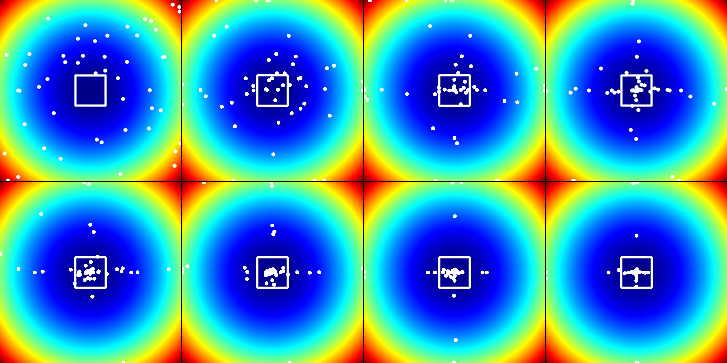
\includegraphics[width=1.0\textwidth]{figure/b.png}
\renewcommand\figurename{图}\caption{螺旋收缩位置变换模拟结果}
\end{figure}

图6是螺旋更新位置策略,虽然并没有加入包围的策略,但由于l在[-1,1]随机变化的原因,以及坐标差缩小的概率较大,也呈现出一定的收缩趋势,只不过比包围收缩慢很多。

\subsection{WOA在凸函数上的搜索过程模拟结果}
在本节中,通过求解一个凸函数$f(x)=max(x_1,x_2)$在$x_1$、$x_2$属于[-1,1]之间的最小值,展示WOA三种位置更新策略混合作用下的搜索过程。鲸鱼数目为25条,每次迭代的鲸鱼位置如图7。
\begin{figure}[H]
\centering
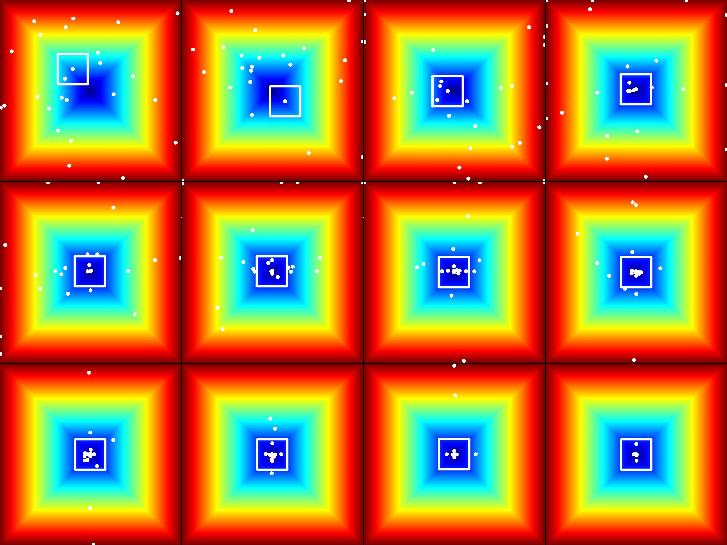
\includegraphics[width=1.0\textwidth]{figure/c.png}
\renewcommand\figurename{图}\caption{WOA在凸函数上的搜索过程模拟结果}
\end{figure}

可以看到,中间方框的局部最优解逐步收缩到中心的全局最优解,在第10代到11代时,可以看到仍有鲸鱼跑到外面去探索更优的解,可见WOA具备一定跳出局部最优的能力。

\subsection{WOA在非凸函数上的搜索过程模拟结果}
在本节中,通过求解两个非凸函数$f(x)=4x_1^2-2.1x_1^4+x_1^6/3+x_1x_2-4x_2^2+4x_2^4$ 、$f(x)=x_1^2-10cos(2\pi x_1)+x_2^2-10cos(2\pi x_2)+20$ 在x1、x2属于[-1,1]之间的最小值,展示WOA三种位置更新策略混合作用下的搜索过程。鲸鱼数目为25条,每次迭代的鲸鱼位置如图8。
\begin{figure}[H]
\centering
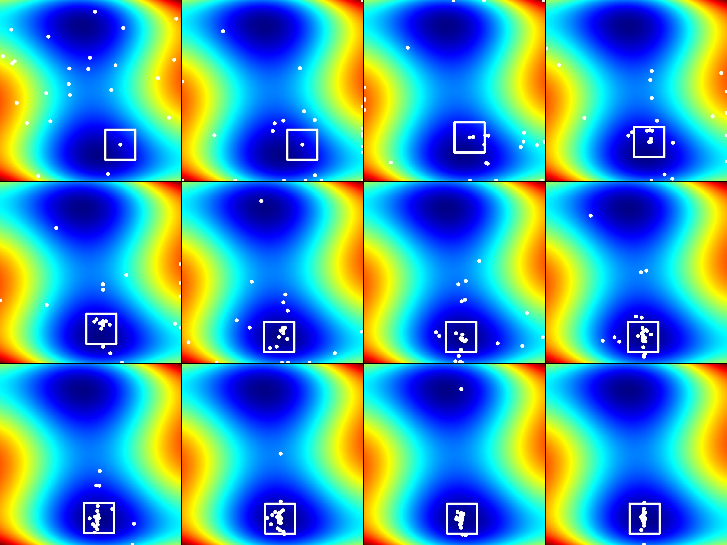
\includegraphics[width=1.0\textwidth]{figure/d.png}
\renewcommand\figurename{图}\caption{WOA在非凸函数1上的搜索过程模拟结果}
\end{figure}

图8可以看到,在两个全局最优解中,算法收敛到了下面一个全局最优解附近,还是第9--11代,探索阶段的策略仍起到了很好的探测局部最优解外面的解空间的效果。
\begin{figure}[H]
\centering
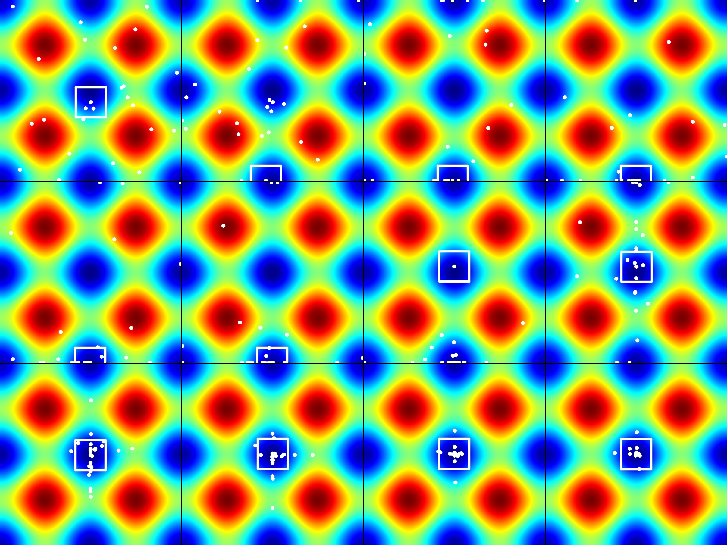
\includegraphics[width=1.0\textwidth]{figure/e.png}
\renewcommand\figurename{图}\caption{WOA在非凸函数2上的搜索过程模拟结果}
\end{figure}

在这个函数中,只有中间的深蓝色是全局最优解。可以看到,WOA在运行过程中,首先1~6代由向下面一个局部最优解收敛的趋势,但由于第7代一条鲸鱼变换到了中间全局最优解的附近,使得所有其他陷于局部最优的鲸鱼都朝他包围收缩或螺旋变换位置,最终收敛到了全局最优解的附近。

\section{评价}
通过模拟程序,可以看到在WOA算法中:包围收缩是一个快速版的收缩过程,螺旋变换是一个慢速的收缩过程,而随机探索是一个跳出局部最优的主要手段。这三种过程相互配合生效的主要假设是局部最优解的附近有全局最优解,因此对于局部最优和全局最优在空间上差距不大的情况下,能有很好的收敛速度。而对于某些极为苛刻的非凸函数,则需要较长时间的随机探索才能收敛到全局最优解附近。因此针对各种实际情况,合理分配这三种过程发生的频率,才能让WOA算法发挥最佳的性能。

\section{参考文献}
Mirjalili S, Lewis A. The Whale Optimization Algorithm[J]. Advances in Engineering Software, 2016, 95:51-67.

\end{document}